


\section{Techniques for Mining Unstructured Text}
\label{cp2:general-approaches}




In this section, we provide background information on general 
approaches used
by software engineering researchers 
to identify text in natural language software artifacts~\cite{Bavota2016}.
We focus on 
automated approaches that might assist a person in discovering
text that addresses an information need,
presenting both core concepts needed to understand an approach 
and seminal work that has used an approach in 
the context of natural language software artifacts.



% For each approach, we detail 
% present seminal work that has applied 
% these approaches to problems related 
% to software engineering.
% These studies focus on specific tasks such as finding relevant passages in API documentation~\cite{Maalej2013,
% Petrosyan2015, Robillard2015}, learning about API types in code tutorials~\cite{Jiang2016b, Jiang2017},
% or detecting sentences that discuss a bug's expected behaviour~\cite{Chaparro2017}.
% These approaches respectively use the presence of code words, HTML anchor links, or whether a sentence contains
% a modal verb as properties to automatically identify relevant text.




\subsection{Pattern Matching}
\label{cp2:pattern-matching}



Pattern matching approaches use regular expressions describing
a sequence of tokens that represent
the text to be identified~\cite{Bavota2016}. 
We have shown how pattern matching identified
books whose subject contained
the keyword `\textit{android}' (Figure~\ref{fig:library-catalogue})
and the same principle could assist 
in finding parts of an artifact that contain some keyword, 
as many web browsers allow via a `\textit{find in page}' feature (Figure~\ref{fig:find-in-page}).
Nonetheless, this support is very limited and users would have to manually
inspect each match to 
determine if they are relevant or not.






\medskip
\begin{figure}[h!]
    \centering
    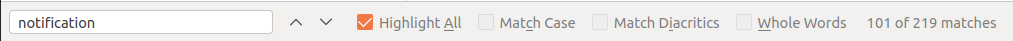
\includegraphics[width=\textwidth]{cp2/find.png}
    \caption{Find in page feature with results for the `\textit{notification}' term}
    \label{fig:find-in-page}
\end{figure}


More automated approaches have also been built using pattern matching, 
as when Panichella et al. 
matched class elements mentioned in development mailing 
 lists to source code files
to assist developers in finding information useful to 
 understanding the source code~\cite{panichella2012}.
Although the heuristics and regular expressions used in this and other studies (e.g.,~\cite{nadi2020, Maalej2013})
are lightweight and effective~\cite{Bavota2016}, 
pattern-matching approaches 
are often specific to certain kinds of domains and types of artifact~\cite{fucci2019}, 
limiting their use in the design of a generalizable technique.


% In development mailing lists, Panichella et al. 
% proposed an automatic approach leveraging \acf{IR} to extract 
% text with useful information that assists in understanding code elements inspected by a developer~\cite{panichella2012}




\subsection{Information Retrieval }
\label{cp2:information-retrieval}


% \red{The IR section in the related work needs some re-positioning. It doesn’t really flow in making an argument or situating IR.}

% Such a definition encampsulates }
% techniques
% or approaches for finding documents, paragraphs, sentences, etc. 
% that satisfy an information need ()~\cite{manning2010IR}.

\acf{IR} comprises \rev{the structure, analysis, storage, search, and retrieval of information~\cite{salton1983} and it has many sub-fields~\cite{zhang2016, liu2019data, tamine2010}, including: 
\textit{ad-hoc retrieval} referring to the basis upon which an IR system strives to return an accurate set of documents relevant to an input query;
\textit{question answering} referring to finding answers to an input question; and
\textit{contextual retrieval} referring to finding information based on a particular context, such as a user's task.}


% \rev{


\rev{
Among these sub-fields, the work in this thesis is closer to contextual retrieval, where multiple attributes model context, such as a user's intentions, tasks, needs, and the environment in which information activities occur~\cite{dourish2004we}. For example, a contextual-aware \acs{IR} system could provide different recommendations 
based on a user's age~\cite{kofod2003case}.} 



\rev{If we focus on `task context', the information available on a software task can serve as a starting point to an input query, where} classical \acs{IR} systems use the frequency or co-occurrence of words (or phrases) to determine the relevance of an artifact for that input query.




Given a set of words in an input query,
\acs{IR} finds which artifacts contain that word, or where within an artifact it appears
and, based on this principle, multiple \acs{IR} schemes have been proposed 
to identify text based on 
how not all the words in some vocabulary have the same weight (\textit{TF-IDF})~\cite{luhn1957tf, jones2004idf}, 
how to  represent sentences (\textit{VSM})~\cite{Salton1975vsm}, 
or how to account for different words that appear interchangeably in some context (\textit{LSI})~\cite{dumais1994latent}. \rev{We discuss other and more complex schemes using \acf{NLP}, \acf{ML}, or \acf{DL} in later sections of this chapter.}




In natural language software artifacts, 
information retrieval has been used 
as part of approaches that
automatically identify sentences  that a developer would first read in a bug report 
when pressed with time~\cite{Lotufo2012},
or in approaches that help cluster software components to aid program comprehension of a software system~\cite{Marcus2003}.
In this dissertation, we combine information retrieval and word embeddings 
to identify relevant text across different kinds of artifacts, as Chapter~\ref{ch:identifying} further details.

    

% 




\subsection{Natural Language Processing }
\label{cp2:nlp}


\acf{NLP} relies on the lexical or syntactical analysis of the text~\cite{jurafsky2014speech}
and such analyses might assist in the automatic identification of text that satisfies an information need. 
To illustrate some of the elements obtainable using \acs{NLP}, we consider a short sentence 
instructing how to perform a file system operation: ``\textit{you can use io.StringIO}''.
Figure~\ref{fig:nlp-analysis} shows elements extracted for this sentence using two \acs{NLP} techniques,
namely \acf{POS} tagging and dependency parsing.
The former assigns tags\footnote{\url{https://cs.nyu.edu/~grishman/jet/guide/PennPOS.html}} ({\small \textit{PRP}, \textit{VP}, \textit{NNP},} etc.) to each word 
in a sentence~\cite{taylor2003penn} while the latter identifies
relationships between them, such as how 
`\textit{io.StringIO}' is the direct object (\textit{obj})
associated with the verb `\textit{use}'.



\begin{figure}[h!]
    \centering
    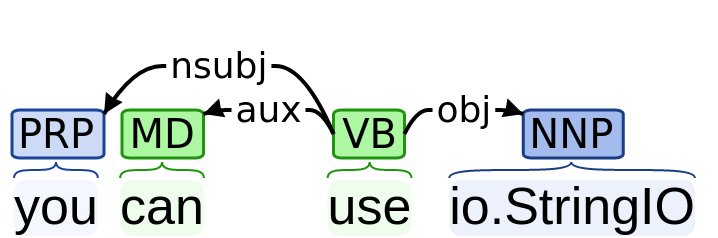
\includegraphics[width=0.40\textwidth]{cp2/textual-analysis.png}
    \caption{Syntactic elements for a sentence giving instructions about how to perform some file system operation}
    \label{fig:nlp-analysis}
\end{figure}


As an example of the application of \ac{NLP} to software engineering text,
Robillard  and Chhetri proposed a tool (Krec)
that uses \acs{POS} tagging to automatically 
identify text with threats and directives on how to use some API element~\cite{Robillard2015}.
As another example, {\small DeMIBuD}
is an automatic approach that uses dependency parsing
to automatically detect sentences discussing a bug's expected behaviour~\cite{Chaparro2017}.
In this work, we use \acs{NLP} as part of our 
analysis of the text deemed relevant to a set of software tasks (Chapter~\ref{ch:characterizing}).



\subsection{Machine Learning }
\label{cp2:machine-learning}



Several other studies have investigated the text 
of various kinds of natural language artifacts and 
the meta-data available on them~\cite{Ko2006, Maalej2013, Arya2019}.
Findings arising from these empirical studies
indicated regularities in the text and meta-data of 
an artifact which could be engineered into 
features that a  \acf{ML} technique could use to automatically identify or classify
text that addresses certain information need~\cite{Bavota2016}. 



Machine learning techniques can be categorized 
according to how they make use of available data. 
Supervised learning approaches use a set of features and labeled data
to train classifiers for detecting entities of interest (e.g., text, images, etc.)
while unsupervised learning approaches do not require labeled data and 
identify entities according to properties inferred from the data.



\subsubsection{Supervised Learning }
\label{cp2:supervised}


With regards to supervised learning approaches, 
we consider the families of classifiers that 
determine
\textit{(1)} if some entity belongs or not to a given class, as in binary classification
\textit{(2)} which class, out of many, some input entity belongs to, as in multinomial classification, or
\textit{(3)} which classes can be assigned to a given input, as in multi-label classification~\cite{alpaydin2020ml},
 and we detail their application to software engineering problems.



% Binary classifiers can be expressed as functions in the form of 
% $f(x) \arrowkeyright y$, where $x$ is a vector of features and $y \in {1, 0}$.
% Hence, it indicates whether $x$ belongs or not a given class.



Among other applications, binary classifiers have been used 
to classify text in bug reports that describes (or not) steps to reproduce a bug~\cite{Chaparro2016}
or  to classify paragraphs which contain explanations 
about API elements in a web tutorials~\cite{Petrosyan2015}.
In turn, multinomial classifiers have been mostly used 
to identify a category, out of many, that represents the type of information 
associated with some text. For instance, Arya et al. identified 16 categories of  information available
in open source GitHub issues (e.g., workarounds, solution discussion, task progress, etc.)
and they proposed a multinomial classifier 
to automatically identify such categories~\cite{Arya2019}.
In a similar manner, Fu and colleagues consider 
five types of decisions that might arise during 
email exchanges (e.g., design, testing, management decisions, etc.)
and they proposed a multilabel classifier 
to automatically identify all the decisions present in emails of
a development mailing list~\cite{fu2021}.





Regardless of the type of classifier, these approaches are typically built 
with training data containing human-engineered features and the cost and effort of hiring skilled workers to produce 
the labeled data for these and other supervised learning approaches
has been a major limitation to their usage in software engineering research~\cite{Arpteg2018, ferreira2021}.




\subsubsection{Unsupervised Learning}
\label{cp2:unsupervised}



Common applications of unsupervised learning 
to natural language software artifacts 
comprise text summarization~\cite{Goldsteinet1999} and data clustering, which might help an individual both in understanding the key information in an 
artifact and also in deciding which information patches are 
 worth their time~\cite{Lotufo2012}.


Unsupervised summarization approaches are often based on 
variations of the PageRank algorithm~\cite{Page1999}, and these approaches identify
the most central sentences in an artifact based on a set of relationships
established between all the sentences in that artifact.
Among other natural language artifacts,
extractive summarization techniques
have been applied to Stack Overflow posts~\cite{Ponzanelli2015},
coding tutorials~\cite{Li2018},
or bug reports, as
when Li et al. summarized 
key elements required to understand a bug and its resolution~\cite{li2018deep}.




A second family of unsupervised techniques focuses on clustering data.
These techniques use properties or features in the data to 
identify 
subsets with similar characteristics. 
Techniques that cluster data, such as \acf{LDA}~\cite{blei2003latent},
have been used by software engineering researchers to both 
bootstrap the categorization of information in 
natural language artifacts and as part of tools that identify topics in the text. 
For instance, Allamanis and Sutton
applied \acs{LDA}
to gain insight into the types of questions 
asked on Stack Overflow~\cite{Allamanis2013}
while FRAPT is a tool that 
uses \acs{LDA} to identity topics in a web tutorial
as well as relevant sentences in each of the topics identified~\cite{Jiang2017}.



Although unsupervised techniques lift the need for labeled training data,
they still use human-engineered features, 
which are often specific to certain 
types of artifact. Therefore, 
both supervised and unsupervised machine learning techniques
have limitations that might prevent their usage 
in the design of a generalizable technique.




\subsection{Deep Learning }
\label{cp2:deep-learning}



In contrast to the human-engineered features,
\acf{DL} approaches allow the automatic extraction of features 
from training data through a set of mathematical transformations~\cite{Deng2018, zhang2021deep}.
This makes 
deep learning an interesting 
approach to
uncover regularities 
that are not obvious or easily identified
by feature engineers or researchers.



A common application of \acs{DL} in software engineering is the usage of neural, or word, embeddings~\cite{Mikolov2013}
for information retrieval purposes. 
Neural, or word, embeddings produce vector representations in a continuous space,
where words with similar meanings are typically close in the vector space~\cite{harris1954distributional, mikolov2013efficient}. 
Researchers have found that word
embeddings mitigate lexical mismatches in the text found across different 
natural language software artifacts,
as shown by Ye et al.'s evaluation of word embeddings
for bug localization~\cite{Ye2016}
or Huang and colleagues' study on 
the usage of word embeddings for API recommendation~\cite{Huang2018}.
Guided by these findings, Chapter~\ref{ch:identifying} describes 
how we use word embeddings in the identification 
of task-relevant text.



Many other \acs{DL} studies in software engineering~\cite{ferreira2021,li2018deep}
use neural network architectures 
for the same range of problems we presented when discussing machine learning techniques for mining unstructured text (Section~\ref{cp2:machine-learning}).
As explained by Watson et al.~\cite{watson2022},
neural network architectures are composed of several layers 
that perform a series of transformations on data passing through them. 
A set of parameters controls these transformations and 
adjust the model being trained so that it can predict 
the right outcome for any given input.
Using these concepts, researchers have proposed 
several  \acs{DL} architectures (e.g., \acs{RNN}s~\cite{rumelhart1986rnn, sutskever2014seq2seq}, encoder-decoders~\cite{bahdanau2014neural}, Transformers~\cite{Vaswani2017attention}, etc.) 
suitable for different problems. 
For instance,
Li et al. used an auto-encoder~\cite{liou2014autoencoder}
to produce more accurate and diverse summaries 
for bug reports~\cite{li2018deep} while 
Fucci et al. used a 
recurrent neural network (\acs{RNN}) 
to identify the types of information available in 
API documentation~\cite{fucci2019}.

% with \acf{LSTM}~\cite{hochreiter1997lstm}


Similar to supervised \acs{ML} approaches, deep learning approaches 
typically require large amounts of data for training purposes.
Nonetheless, recent advancements on the usage of
pre-trained models 
have lifted some of these limitations~\cite{erhan2010pre-train}.
In Chapter~\ref{ch:identifying},
we investigate how we can use a state-of-the-art architecture, namely BERT~\cite{Devlin2018Bert},
to identify relevant text across different types of artifacts.




% \subsection{Summary of Techniques}


% \art{Should I have a summary section and a table bundling examples of studies for each technique and the artifacts that they apply to? }






% Researchers pose the problem of identifying text 
% in a natural language artifact 
% as a binary classification problem. 
% That is, the use of a number of features 
% to predict whether the text is (or not)
% relevant to some context~\cite{aa}.
% In software engineering, 
% binary classifiers have been used for,
% for example, classify text that describes steps to reproduce a bug~\cite{Chaparro2016} or 
% classify text that explains a certain API element, as when 
% Petrosyan et al. used 
%  sentence-level features
% and meta-data features in a classifier 
% that 
% identifies explanations about an API element  in a web tutorial~\cite{Petrosyan2015}.




% Other classification problems predict which class, out of many, some input text belongs to. 
% This type of classification, referred to as multinomial or multi-class classification, 
% is of particular interest if 
% we consider the taxonomies described in Section~\ref{cp2:text-in-se}.
% For example, Arya et al. identified 16 categories of  information available
% in open source GitHub issues (e.g., workarounds, solution discussion, task progress, etc.)~\cite{Arya2019}
% and they proposed a multinomial classifier 
% to automatically identify such categories.








% Although valuable, these classifiers are instances of supervised learning methods.
% They require training data so that a classifier predicts the correct outcome 
% and the cost and effort of hiring skilled workers to produce 
% the labeled data for these and other supervised learning approaches
% has been a major limitation to their usage in software engineering research~\cite{Arpteg2018, ferreira2021}. As an alternative,
% researchers have also explored 
%  unsupervised learning methods---\acs{ML} techniques that do not required training data---for the automatic 
% identification or classification of the text in natural language artifacts~\cite{aa}.





% A common application of unsupervised learning in software engineering
% considers the automatic generation of text summaries.
% Most often, automatic summaries are produced 
% using extractive techniques that select a subset of 
% the sentences of an artifact that will compose the summary~\cite{a}.
% Among other natural language artifacts,
% extractive summarization techniques
% have been applied to Stack Overflow posts~\cite{a}, coding tutorials~\cite{a},
% or bug reports, as
% when Lotufo et al. 
% considered the kinds of sentences a developer would find relevant 
% to understand a bug report when pressed with time~\cite{Lotufo2012},
% and proposed an unsupervised summarization approach 
% based on the PageRank algorithm~\cite{Page1999}
% to identify these sentences. 




% A second set of unsupervised methods focus on clustering data.
% These techniques identify 
% subsets in the data that have similar properties or features 
% and techniques such as \acf{LDA}~\cite{blei2003latent}  have been used both to 
% bootstrap the categorization of information in 
% natural language artifacts and as part of tools that identify 
% portions of the text in an artifact that are helpful to some context. 
% As an example of the former, 
%  Allamanis and Sutton
% applied \acs{LDA}
% to gain insight into the types of questions 
% asked on Stack Overflow~\cite{Allamanis2013}.
% For the latter, tools such as FRAPT
% use \acs{LDA} to identity topics in a web tutorial
% and then extract sentences explaining API elements from each of the topics identified~\cite{Jiang2017}.


% Despite the significant contributions of these and other studies,
% one substantial challenge inherent to the supervised and 
% unsupervised \acs{ML} approaches 
% is that researchers must engineer which 
% features their \acs{ML} technique will use~\cite{ferreira2021}.
% Hence, \acs{ML} approaches have limitations similar to the pattern 
% matching approaches when we consider 
% the specificity and cost of engineering such features
% for a variety of kinds of artifacts.








% pre-trained models that do not require large amounts of training data to our domain problem~\cite{devlin2018bert, Ye2016}. With this approach, we revisit findings on the trade-offs of using machine learning techniques to mine textual data~\cite{Chaparro2017, Bavota2016}.




% using them as a way to compare the semantic similarity of the text~\cite{mihalcea2006}.
% Guided by the recent success of word embeddings 
% for a variety of software development 
% activities,,
% Chapter~\ref{ch:identifying} 
% describes how we incorporate word embeddings in the 
% design of techniques that automate the identification of task-relevant text. 






% ,
% thus allowing \acs{DL}
% to automate the identification of text in natural language software artifacts
% with these `hidden' properties. 









% These studies focus on specific tasks such as finding relevant passages in API documentation~\cite{Maalej2013,
% Petrosyan2015, Robillard2015}, learning about API types in code tutorials~\cite{Jiang2016b, Jiang2017},
% or detecting sentences that discuss a bug's expected behaviour~\cite{Chaparro2017}.
% These approaches respectively use the presence of code words, HTML anchor links, or whether a sentence contains
% a modal verb as properties to automatically identify relevant text.
% Given how quickly developers progress to using new kinds of technology to
% record pertinent information (e.g., slack~\cite{Storey2017, Lin2016}),
% it may be difficult to scale such artifact-centric approaches to cover the range of
% artifacts that could be returned from a search.
% A second issue arises from the fact that coding procedures used to determine relevancy
% in these studies do not consider disagreements~\cite{Stol2015}.
% That is, there are many criteria in how individuals
% assess relevance~\cite{Barry1994, Barry1998, Freund2015}
% and there are no guarantees that
% developers will use the same properties to determine text relevant to their tasks~\cite{Freund2013, Freund2015}.
% In contrast, our study does not pre-assume any relevance cues, and instead,
% we leave the decision of what text is perceived as relevant to a particular task to
% the participants in our experiment.









% Knowledge Recommender ()
% is an example of a
%  tool that uses lexical patterns to 
%  automatically detect relevant text in  API documentation. 
% Krec's premise is that relevant sentences contain a code element, such as a method or class signature.
% These code elements are identifiable via regular expressions 
% and Krec contains a catalog of 361 unique patterns 
% that identify threats and directives on how to use some API element.
% For example, Krec uses the pattern {\small \textit{$\{$may}, \textit{efficient}, \textit{code element regex$\}$}} 
% to identify sentences giving instructions about an efficient way to 
% perform some operation. 



%  is a linguistic-based approach that 

% It uses a set of 154 discourse patterns
% derived from nearly 3,000 bug reports 
% to identify such sentences. 
% For example, the pattern 
% {\small \textit{$\{$subject}, \textit{should/shall (not)}, \textit{complement$\}$}}
% captures common ways with which developers describe a system's expected behaviour
% and empirical assessment of the patterns used by the tool has shown that it 
% detects sentences of interest in bug reports with high accuracy.



% ~\cite{krallinger2017}



% ~\cite{mcdonough2019}